\documentclass[
]{beamer}

\usepackage[english]{babel}
\usepackage[utf8]{inputenc}
\usepackage[T1]{fontenc}
\usepackage{lmodern}
\usepackage{csquotes}
\usepackage{expl3,biblatex}
\addbibresource{main.bib}
\usepackage{booktabs}
\usetheme[
  workplace=fi,
  fonts=none,
]{MU}
\usepackage{textalpha}
\usepackage{subfigure}
\usepackage{wrapfig}
\usepackage{tikz}
\usepackage{appendixnumberbeamer}

\title[Visualisation and Annotation of VolSeg Data in Mol*]{Lightweight Visualisation and Annotation of Volumetric and Segmentation Data in Mol*}
\subtitle[Master's Thesis Defense]{Master's Thesis Defense}
\author[D. Tichý]{Dominik Tichý\texorpdfstring{\\}{, }Supervisor: RNDr. Tomáš Raček, Ph.D.}
\institute[FI MU]{Faculty of Informatics, Masaryk University}
\date{February 2, 2025}
\subject{Presentation Subject}
\keywords{Mol*, Mol* VS, MolViewSpec, MolViewStories, volumetric data, segmentations, visualization, bioinformatics}

\begin{document}

\begin{frame}[plain]
\maketitle
\end{frame}

\section[Short Section 1 Name]{Full Section 1 Name}
\subsection[Short Subsection 1 Name]{Full Subsection 1 Name}

\begin{frame}{Motivation}
\end{frame}

\section[Short Section 2 Name]{Full Section 2 Name}
\subsection[Short Subsection 2 Name]{Full Subsection 2 Name}

\begin{frame}{Goals}
\end{frame}

\section[Short Section 3 Name]{Full Section 3 Name}
\subsection[Short Subsection 3 Name]{Full Subsection 3 Name}

\begin{frame}{Solution}
\end{frame}

\section[Short Section 4 Name]{Full Section 4 Name}
\subsection[Short Subsection 4 Name]{Full Subsection 4 Name}

\begin{frame}{Conclusion}
  \begin{itemize}
    \item conversion library
    \item web application
    \item contributed to the design of the new version of Mol* VS
  \end{itemize}
\end{frame}

% \section{\bibname}
% \begin{frame}[t, allowframebreaks]{\bibname}
% \printbibliography[heading=none]
% \end{frame}

\begin{frame}[plain,noframenumbering]
  \begin{tikzpicture}[remember picture,overlay]
    \node[inner sep=0pt] at (current page.center) {
        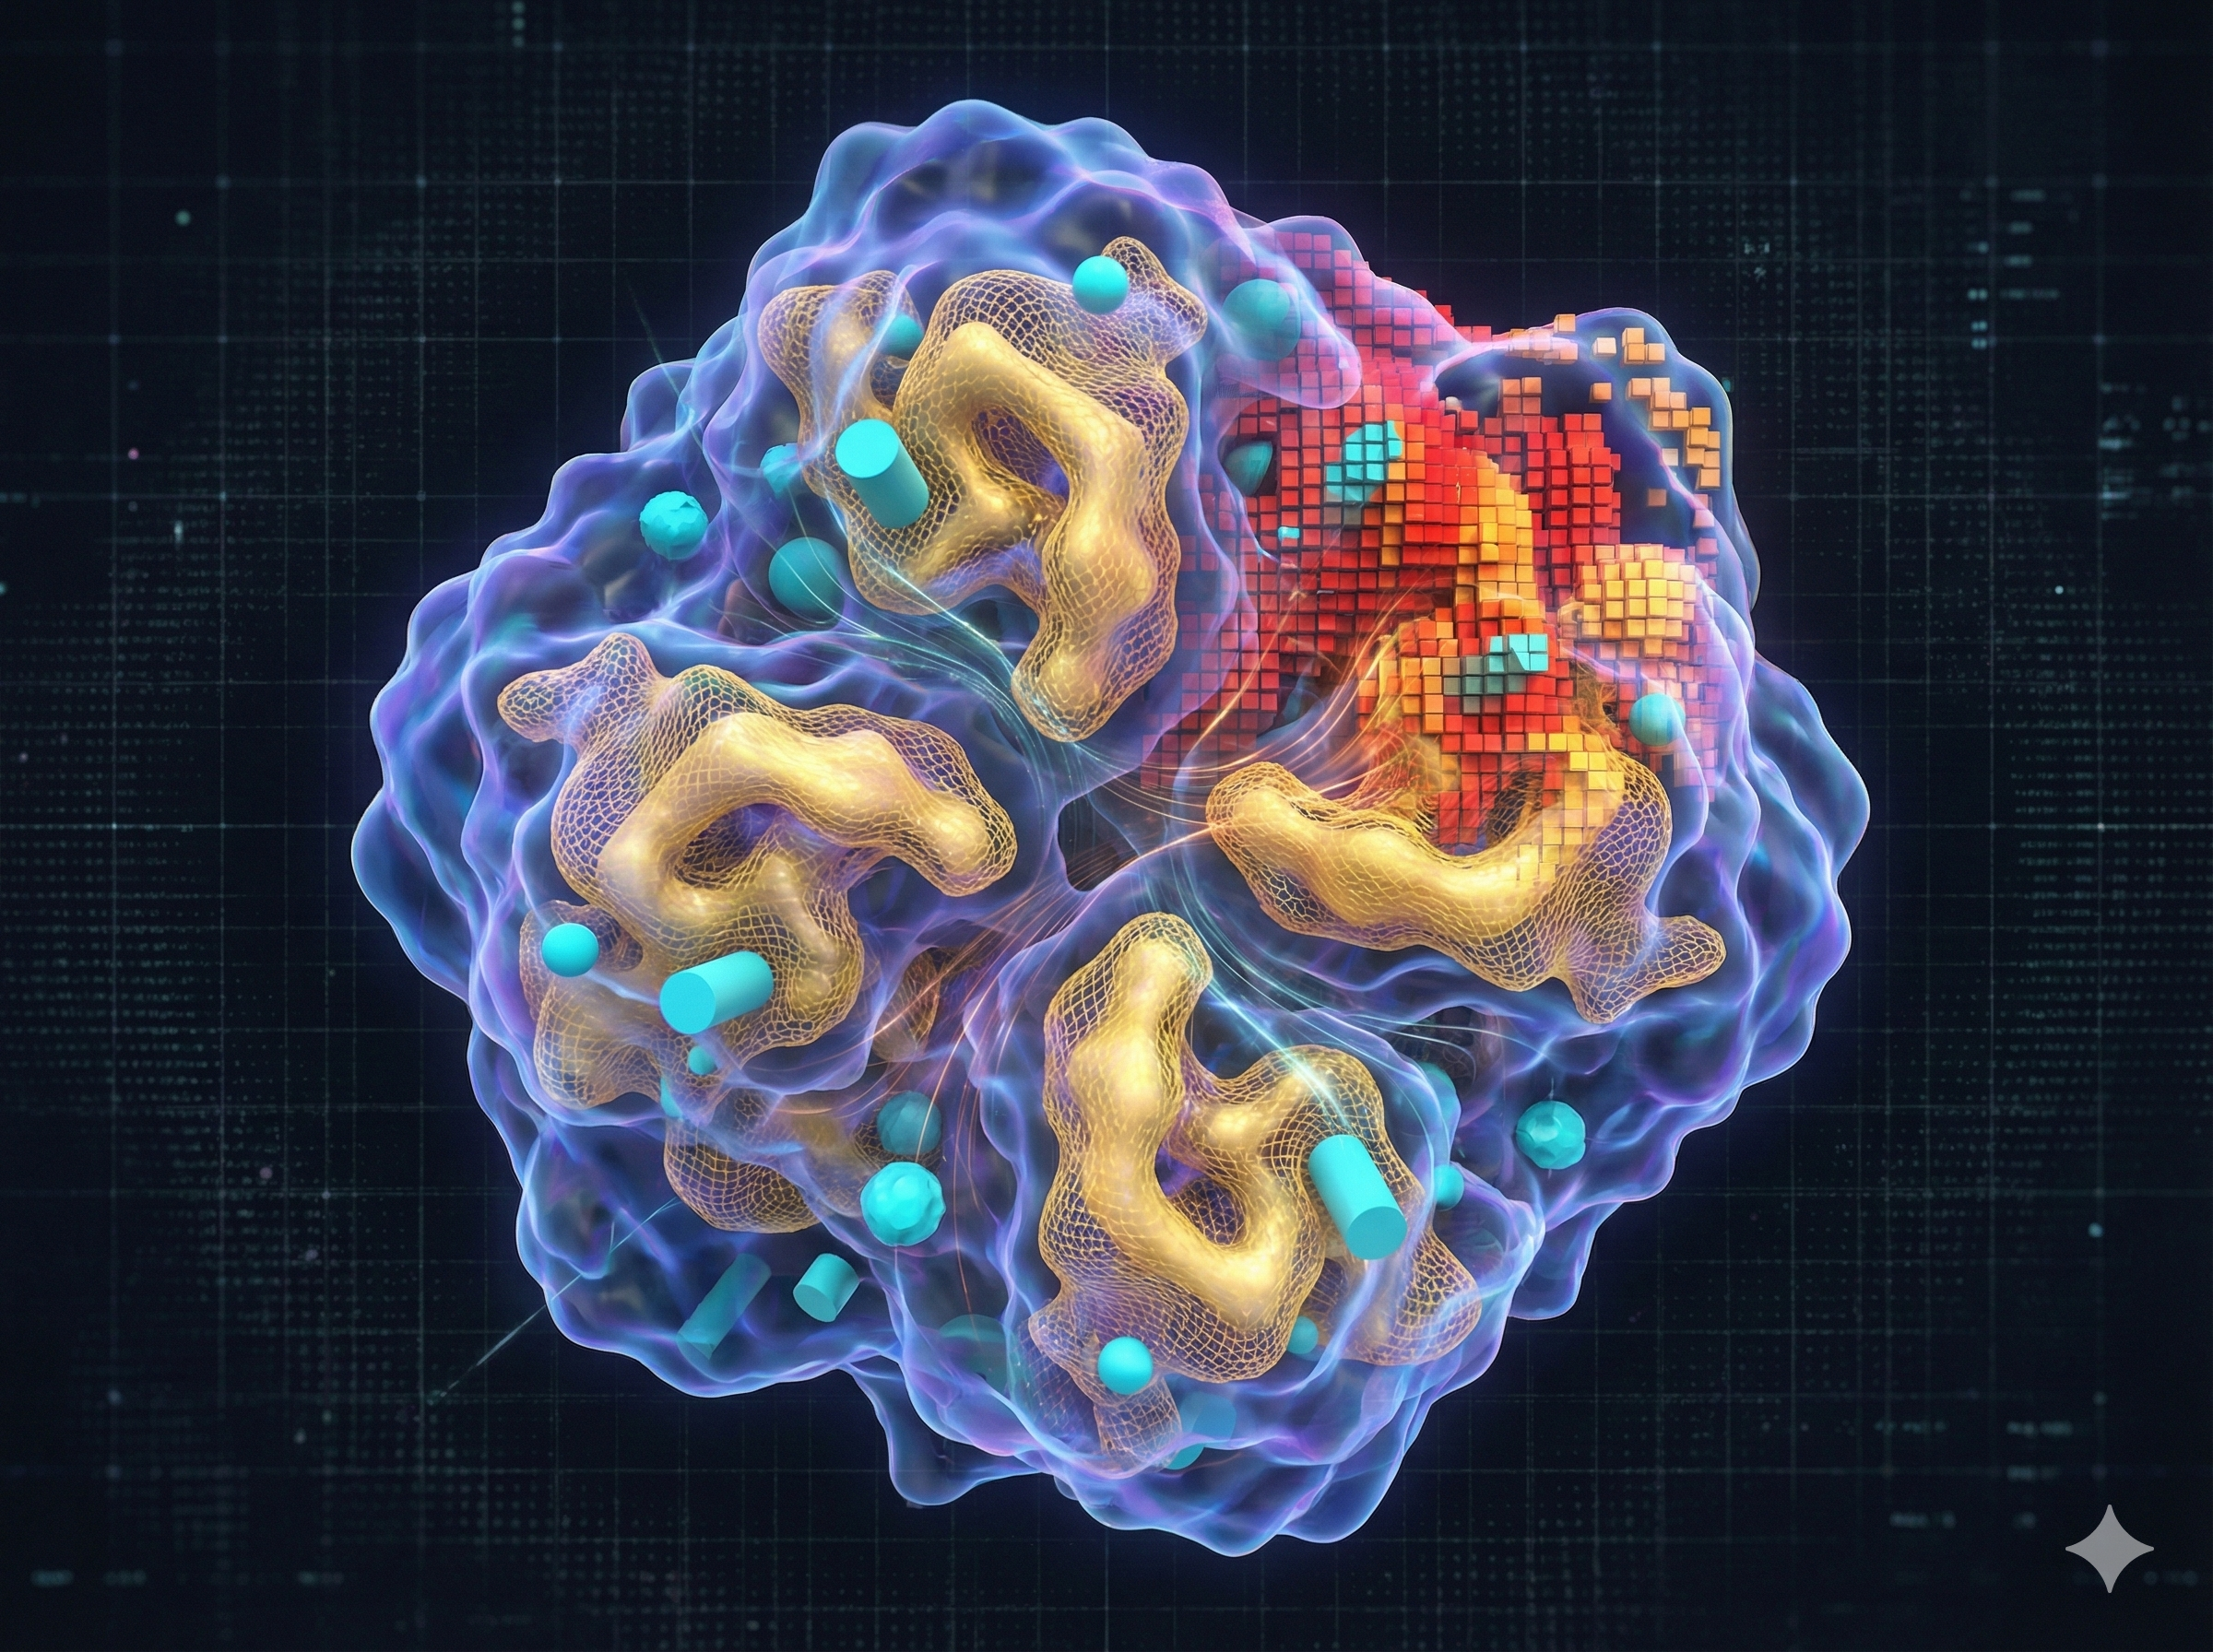
\includegraphics[width=\paperwidth,height=\paperheight]{images/thank-you.png}
    };
    \node[text=white, font=\Huge\bfseries, align=center] at (current page.center) {
        Thank You for Your Attention!
    };
  \end{tikzpicture}
\end{frame}

\appendix

\section{Otázky oponenta}

\subsection[Otázka 1]{Otázka 1}

\begin{frame}
  \begin{block}{Otázka oponenta 1}
    TODO
  \end{block}
  \begin{itemize}
    \item answer
    \item answer
  \end{itemize}
\end{frame}

\subsection[Otázka 2]{Otázka 2}

\begin{frame}
  \begin{block}{Otázka oponenta 2}
    TODO
  \end{block}
  \begin{itemize}
    \item answer
    \item answer
  \end{itemize}
\end{frame}

\subsection[Otázka 3]{Otázka 3}

\begin{frame}
  \begin{block}{Otázka oponenta 3}
    TODO
  \end{block}
  \begin{itemize}
    \item answer
    \item answer
  \end{itemize}
\end{frame}

\makeoutro
\addtocounter{framenumber}{-1}

\end{document}
